%%\documentclass[11pt]{article}

%% Template for a preprint Letter or Article for submission
%% to the journal Nature.
%% Written by Peter Czoschke, 26 February 2004
%%

\documentclass{nature}

%% make sure you have the nature.cls and naturemag.bst files where
%% LaTeX can find them

\bibliographystyle{naturemag}

\usepackage{listings}
\usepackage{color}
\usepackage{caption}
%\usepackage{amsthm,amsmath,amssymb}
%\usepackage{multirow}
\usepackage[pdftex]{graphicx}
%\usepackage{subfigure}
%\usepackage{makecell}
%\usepackage{booktabs}
%\usepackage{array}
%\usepackage{fullpage}
%\usepackage{url}
%\usepackage{algorithm}
%\usepackage{algorithmic}
%\usepackage{bm}
%\usepackage{smile}
%\usepackage{mathtools}
%\usepackage{wrapfig}
%\usepackage{lipsum}
%\usepackage{mathrsfs}
%\usepackage{dsfont}
%\usepackage{titling}
%\usepackage{epstopdf}
%\usepackage{multirow}
%
%\usepackage[usenames,dvipsnames,svgnames,table]{xcolor}
%\usepackage[colorlinks=true,
% linkcolor=blue,
% urlcolor=blue,
% citecolor=blue]{hyperref}
%
%\def\skeptic{{\sc skeptic}}
%\newcommand{\sgn}{\mathop{\mathrm{sign}}}
%\providecommand{\norm}[1]{\|#1\|}
%\providecommand{\bnorm}[1]{\big\|#1\big\|}
%\providecommand{\enorm}[1]{| \! | \! |#1| \! | \! |}
%\providecommand{\bemnorm}[1]{\big| \! \big| \! \big|#1\big| \! \big| \! \big|}
%
\renewcommand{\baselinestretch}{1.1}
%
%
%\def\skeptic{{\sc skeptic}}
%\providecommand{\norm}[1]{\|#1\|}
%\providecommand{\bnorm}[1]{\big\|#1\big\|}
%\providecommand{\enorm}[1]{| | |#1| | |}
%\providecommand{\bemnorm}[1]{\big| \big| \big|#1\big| \big| \big|}
%
%\newcommand*{\Sc}{\overline{\cS}}
%\newcommand*{\Ac}{\overline{\cA}}
%\newcommand*{\Bc}{\overline{\cB}}
%\newcommand*{\supp}{\mathrm{supp}}
%
%\DeclarePairedDelimiter\ceil{\lceil}{\rceil}
%\DeclarePairedDelimiter\floor{\lfloor}{\rfloor}



\usepackage[plain]{fancyref}
\makeatletter
\def\mkfancyprefix#1#2{%
\expandafter\def\csname fancyref#1labelprefix\endcsname{#1}%
% plain lowercase
\begingroup\def\x{\endgroup\frefformat{plain}}%
    \expandafter\x\csname fancyref#1labelprefix\endcsname
    {\MakeLowercase{#2}\fancyrefdefaultspacing##1}%
% plain uppercase
\begingroup\def\x{\endgroup\Frefformat{plain}}%
    \expandafter\x\csname fancyref#1labelprefix\endcsname
    {#2\fancyrefdefaultspacing##1}%
% vario lowercase
\begingroup\def\x{\endgroup\frefformat{vario}}%t
    \expandafter\x\csname fancyref#1labelprefix\endcsname
    {\MakeLowercase{#2}\fancyrefdefaultspacing##1##3}%
% vario uppercase
\begingroup\def\x{\endgroup\Frefformat{vario}}%
    \expandafter\x\csname fancyref#1labelprefix\endcsname
    {#2\fancyrefdefaultspacing##1##3}%
}
\makeatother

\mkfancyprefix{thm}{Theorem}
\mkfancyprefix{lem}{Lemma}
\mkfancyprefix{prop}{Proposition}
\mkfancyprefix{cor}{Corollary}
\mkfancyprefix{def}{Definition}
\mkfancyprefix{cl}{Claim}
\mkfancyprefix{ss}{Subsection}
\mkfancyprefix{alg}{Algorithm}
\mkfancyprefix{ass}{Assumption}

\title{BrainConductor: An open science platform for the development of
neuroimaging
data analysis tools}

%% Notice placement of commas and superscripts and use of &
%% in the author list

\author{Kevin Lin$^{1*}$,Haixiao Du$^{2*}$, Huazhong
Yang$^2$, Yu Wang$^2$, Han Liu$^3${\color{red}}}

\begin{document}

\maketitle



\begin{affiliations}
\item Department of Statistics, Carnegie Mellon University,
Pittsburgh, PA 15217 USA
\item Department of Electronic Engineering, Tsinghua University, Beijing, China,
100084
\item Department of Operations Research and Financial Engineering, Princeton
University, Princeton, NJ 08544 USA
\item[*] These authors contributed equally to this work
\end{affiliations}

\begin{abstract}
    BrainConductor project is a project parallel to Bioconductor. Like
Bioconductor, BrainConductor is an open platform for sharing neuroimaging data
and R-based data analysis software. BrainConductor aims at promoting
interdisciplinary collaboration between neuroscientists and
statistical scientists, bringing state-of-the-art statistical methodologies and
toolboxes into neuroscience, and enhancing the reproducibility of remarkable
research results. We describe details of our motivations, goals, methods, and
the difference between BrainConductor and related neuroinformatics projects.
Finally, we present some working instances to better explain advantages of
BrainConductor.
\end{abstract}


Modern statistics aims to infer information from high-dimensional data
and has progressed significantly over the last decade.
However, two obstacles currently hinder the
application of these methods to large-scale neuroimaging data
in practice.
First, domain-specific expertise and computational power is needed to handle
the various data file types and to manage the storage
of these large-scale datasets. Second, specialized softwares and
many in-house analysis pipelines have been developed that
prevent new researchers from entering the field.
The BrainConductor project is an open-neuroscience
initiative to address
these obstacles.
As the neuroscience community expands upon open-access
datasets such as the  International Neuroimaging Data-Sharing
Initiative Project (INDI), comparable advances in
open-neuroscience platforms are required
for high
throughput, computationally efficient statistical models
to handle high-dimensional data in this big data era.

%The cooperative trends creates new challenges.
Our goal is to %, and the foremost of all is to
build a knowledge hub and interdisciplinary community by connecting
neuroscientists and statisticians.  Neuroscientists
drive the scientific process by collecting new data and constructing focused
experiments. Non-invasive imaging techniques have gain popularity to
investigate how phenotypic variation
influence the connectivity differences in the human
connectome among individuals\cite{sporns2005human,sporns2011human}. These
include structural and functional MRI,
diffusion tensor imaging (DTI), and Electroencephalography
(EEG).
On
the other hand, statisticians bring new statistical methods
designed to address the high-dimensional, large-scale and complex
data. Such techniques can be divided broadly into
two categories:
summarizing the data (i.e., estimating the brain connectivity, represent
a parcellation of voxels' time series with a single time series)
and uncertainty assessment (i.e., testing for significant difference
between the connectomes of two populations, determining if the
connectivity between two region of interests is due to chance).
We strive to help enable ease of collaboration between these two communities.
While the neuroscientist will benefit from the modern techniques to
analyze these datasets, the statistician
will benefit from the lowered barrier-to-entry
due to the  simplified processes of data acquisition, data management, and data
sharing.


Towards this end, we propose the BrainConductor project, an integration of
high-quality and easy-access datasets, and user-friendly software for both
neuroscientists and statisticians. BrainConductor is a project parallel to
Bioconductor. In the past tens of years,
Bioconductor\cite{gentleman2004bioconductor} made a great contribution to the
progress of
the human genome research because of its transparency, pursuit of
reproducibility, and efficiency of development. Moreover, the open-source
developing architecture of Bioconductor based on R language provides facility to
take advantage of the mature statistical packages rather than re-implementing
functionality. In future neuroimaging studies, an open-source platform is of
necessity to produce collaborative creation of extensible computational tools
and enhance the reproducibility of research results.

This desire has already  %requirement
inspired one of the most prominent projects, Neuroimaging
Informatics Tools and Resources Clearinghouse (NITRC).
NITRC is a resourceful repository collecting popular neuroimaging tools
designed for the preprocessing,
analysis, and display of neuroimaging data, such as
SPM\cite{penny2011statistical}, FSL\cite{jenkinson2012fsl},
FreeSurfer\cite{fischl2012freesurfer} and AFNI\cite{cox1996afni}. NITRC also is
an open repository for many
data sources such as
Alzhelmer's Disease Neuroimaging Initiative (ADNI) and the
1000 Functional Connectome Project (FCP).
However, as successful as NITRC is, there are fundamental
drawbacks from both the developer and user perspectives.
From the developer perspective,
NITRC provides little guidance on effective software
development.
This results in two consequences. First, a large amount of
effort is spent on implementing functions that have
previously been developed by other independent teams. Second,
without establishing an universal file format,
developers on NITRC have to either
write analysis functions for specific file types or spend tremendous
efforts to handle all file types.
For example,
most data sources proffer raw data in the standard industrial DICOM
format, but most of the software packages work on NIfTI or ANALYZE formats.
From the user perspective, there are also key obstacles.
First, software on NITRC are based on different programming models and
processing pipelines and have different interfaces.
Hence, investigators always need lots of training sessions to
learn how to install and use these tools. Second, many statistical
analysis software require a 2D matrix where each covariate
represents a column and each sample represents a row. Since neuroimaging
data is typically represented as a 4D object, new users often
struggle to convert their data into a representation suitable for
most statistical methods. These concerns are summarized in \Fref{fig:nitrc}.

\begin{figure}[tb]
\centering
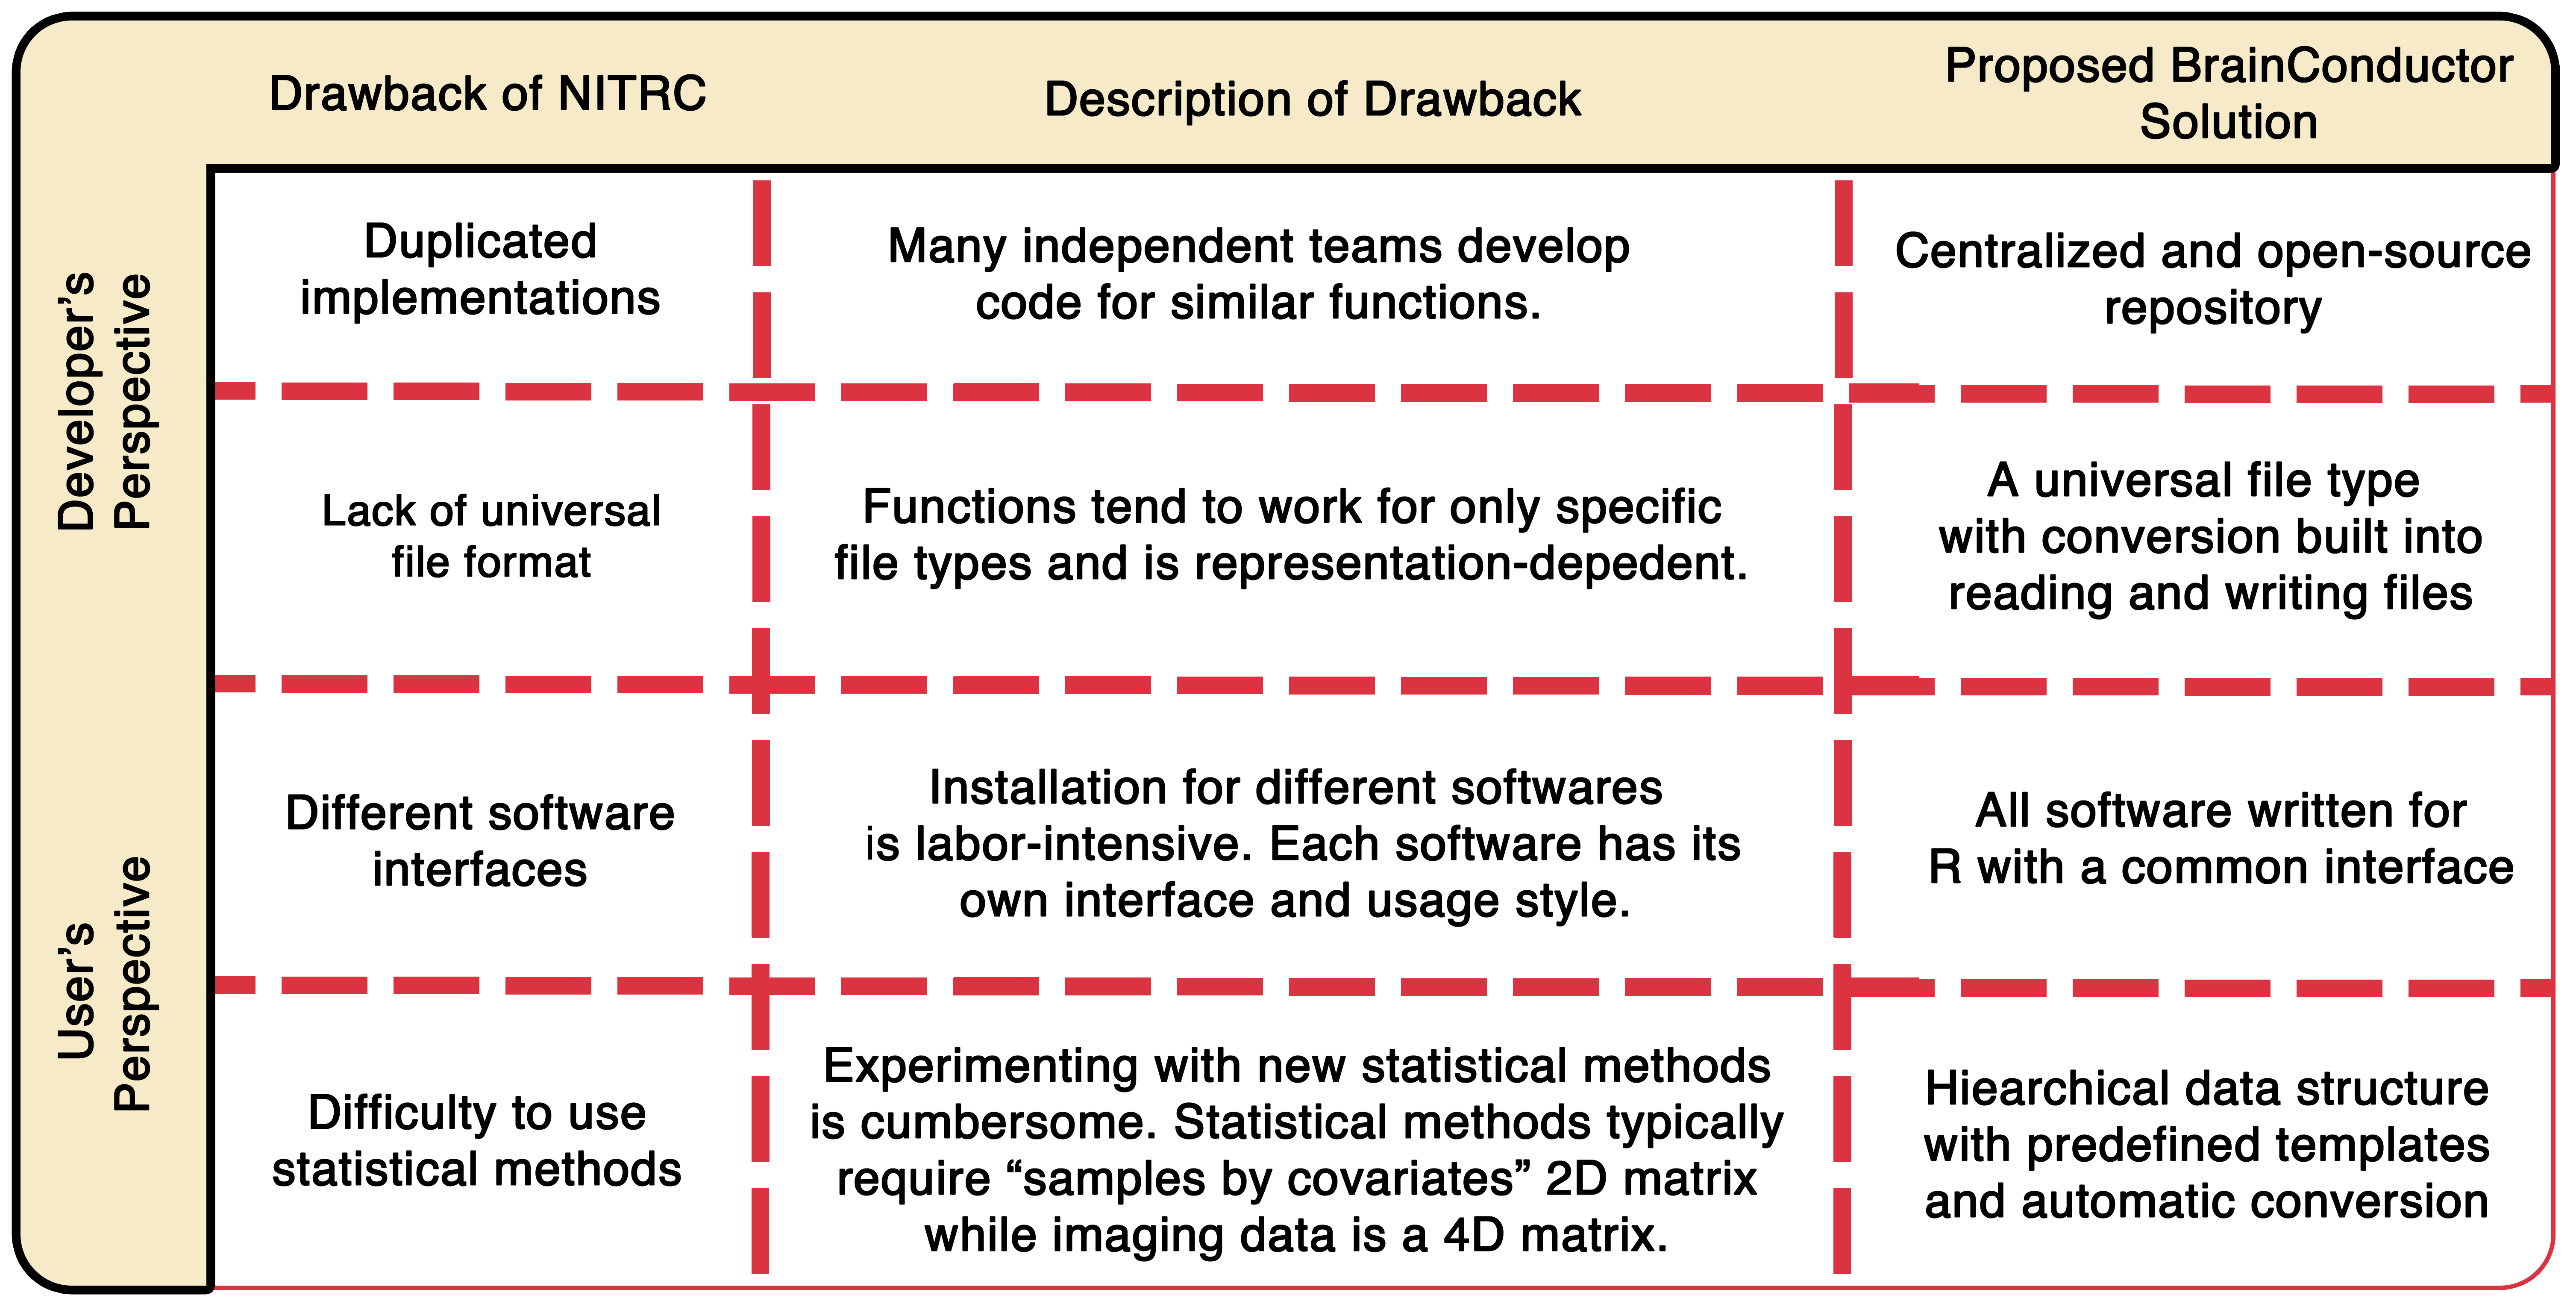
\includegraphics[width=400pt]{fig/brainconductor/brainconductor_nitrc_chart.png}
\caption{Drawbacks of NITRC framework, description of the drawbacks and proposed
solution
in BrainConductor. {\color{red}Need to fix alignment}}
\label{fig:nitrc}
\end{figure}


The BrainConductor project serves two fundamental goals. In connectome-wide
association studies, the goal is to relate differences the macro- and
microarchitecture of the human connectome to phenotypic variation among
individuals\cite{milham2012open}. Towards this end,
in our
initial release of BrainConductor, we focus on an open-neuroscience
solution to manage resting-state fMRI data and study its
subsequent brain connectivity patterns.
In imaging genetics, the ultimate goal
for BrainConductor project is to identify biomarkers and help early diagnosis
for a variety of neuropsychiatric disorders. This will involve a future
integration of genomics and neuroimaging data.


\section{Merits of Computational Strategy}

\subsection{Functionality of R.}
The existing features and communities around a language dictate
its usage and accessibility. As stated before, we are
interested in problems related to data management, mining and analysis
associated with neuroimaging technologies. This orientation requires
a programming environment which is able to foster
efficiency for software development, allowing
streamlined and reproducible research and stimulating
interdisciplinary communication and cooperation.

To meet these requirements, we chose R as the basic programming
modal for BrainConductor project. Our rationale closely follows
the reasons adopted in BioConductor which we summarize
here\cite{gentleman2004bioconductor}.
First, R is an accessible high-level language with
good numerical capabilities allowing quick prototyping of new statistical
computational methods. This allows for a low learning curve for
incoming researchers, rapid experimentation of
new statistical ideas, and a shorter development cycle.
Second, R has a packaging protocol for different software
modules that can be developed individually and distributed easily. The
packaging system of R enables a world-wide collaborative construction of the
Comprehensive R Archive Network (CRAN) with a wide range of
high-quality and well-documented statistical and visualization software
packages. These hundreds of packages are independently developed for specific
objectives, but the objective-oriented programming style of R guarantees the
robust interoperability of packages for more complicated applications. All of
these characteristics of R would decrease development efforts and release time
for reliable software for neuroimaging data analysis.
Third, R also provides
support for high-performance\cite{buckner2010gputools} and parallel
computing\cite{schmidberger2009state},
and interfaces to communicate with specialized code
written in lower-level languages.
Finally, the community of R is
consisted of thousands of active users and developers including biologists,
mathematicians, and engineers. The community provides a natural bridge to
connect the neuroscientists and statisticians. This is much in line with the
intention of the BrainConductor project and is the most important motivation of our
selecting R.


\subsection{Hierarchical Data Structure.} The BrainConductor
project began with significant investment in the infrastructure construction for
software development by formulating the standard for general data structures of
neuroimaging data. A general data structure unifies the interface port and
increases the reusability and interoperability of software packages. The code
written for the analysis of a dataset can be adapted to another similar dataset
since they have the same structure. A researcher doesn't need to modify the code
interface or even write code from scratch.

Currently, the most common file format is NIfTI.
NIfTI is a product of the Data Format Working Group
(DFWG) from the Neuroimaging Informatics Technology Initiative project. It
contains both the header information about the data acquisition
parameters and neuroimaging data as a 4D matrix.
Currently, the oro.nifti R package defines the `nifti'
S4 class in R to manage NIfTI files. However, there are two drawbacks
of this file format that could be encountered by analysts. First, neuroimaging
data files often comprise a large amount of
redundant information.
For example,
the analysis of fMRI data primarily focuses on the gray matter, while the
processing of diffusion weighted MRI focuses on the white matter region.
Therefore, a hierarchical data structure would help save storage and memory
space. Human Connectome Project (HCP) had a similar solution by defining the
CIFTI
file format and grayordinates, a combined cortical surface and subcortical
volume coordinate system\cite{Glasser2013The}.
Second, the NIfTI file format is not flexible for data analytics. Typically,
phenotype information is stored separately in a different file, and many
statistical
methods take as input a 2D matrix organized by samples and covariates.

We define an S4 `NIdata' class based on the NIfTI format
in our Brainbase package as
the general data structure to resolve these problems.
At its core, the NIdata class is a generic file type split into
four slots to store the following information: 1) phenotype
information, 2) specifics of scan sessions, 3) the neuroimaging data
and 4) text-based comments or notes associated with the data that
investigators might document. While we provide an initial structure for storing
phenotype and scan information, users have the flexibility to disregard or
modify these templates before reading the data into R.
Our NIdata format ensures compatibility since most of the conversions from
the existing NIfTI data format are
straightforward. The Brainbase package provides functions
to facilitate
reading in the header information and high-dimensional data array from binary
neuroimaging data files into NIdata class objects.

Most of the engineering of the NIdata class revolved around a more suitable
representation of the neuroimaging data. Like in the CIFTI file
format\cite{Glasser2013The},
we automatically convert all neuroimaging data (a 4D matrix)
into a 2D (potentially sparse) matrix where each
column represents a different voxel
in the brain and each row represents
a different sample from the time series. To ensure that the column indices are
compatible across different NIdata objects, we define generic templates in the
Brainbase packages that dictate which voxel position are assigned to which
columns.
These templates are associated with brain masks and the corresponding tissue
priors.
The NIdata class facilitates the processing
and storage of neuroimaging data based on customizable
templates.
For instance, one of the templates we provide is the MNI 152 brain masks and
tissue priors typically found in FSL.
If users want to keep only voxels corresponding to gray matter, all the column
indices associated with non-gray matter will be `zero'-ed out to save storage.
Moreover, if users want to perform a
region-of-interest or parcellation-based analysis, we provide
additional functions to change the template and perform the data extraction.

To ensure that our 2D representation of neuroimaging data retains the
spatial information of each voxel, the Brainbase package provides
an R S4 object containing the mapping of voxel location to column index and
a list enumerating the column indices of neighboring voxels for each voxel
location. Hence, we can convert our 2D representation back to its original
4D representation to accommodate past software requirements if needed.
Thanks to this flexibility, software developers can
implement algorithms operating directly on the 2D representation in
NIdata without worrying about representation-conversion. {\color{red}Why is this
called ``hierarchical''? I haven't really done anything hierarchical...}

{\color{red}Some concrete numbers of how much memory is saved}
{\color{red}TODO: This code is half-way complete.}

\subsection{File Conversion.}
For developers to write functions using our NIdata class, we need to provide
suitable functions to read different input file types into objects of NIdata class as described in the previous section. Here, We discuss three popular file types in current use, DICOM, NIfTI and ANALYZE.

DICOM is the standard industrial
format for raw data directly collected from an imaging device. The DICOM format
is very broad and very sophisticated. In brief, each .dcm suffix file contains a
number of attributes, including not only the image pixel data but also large
amounts of meta-data information about the subject, imaging devices and settings
during data acquisition.

However, DICOM datasets are redundant, ascribed to the storage of massive
numbers of small files. This is due to each image slice stored as a separate
file. ANALYZE and NIfTI-1 formats are more widely employed in the neuroimaging
community. An ANALYZE format document is composed of one ``hdr" file and one
``img" file. The former contains information about the acquisition settings,
while the ``img" file contain the image data. NIfTI was released as an extension
of the ANALYZE format. The NIfTI data format merges the header and image
information of ANALYZE document into one file (.nii) and enables extending of
the header information. The NIfTI format has alleviated problems with data
storage and sharing across diverse centers, and became one of the most popular
neuroimaging format recently.

BrainConductor offers functions to read all these data format
based on existing software in the oro.dicom and oro.nifti packages. We
provide a generic function that handles all of these file types and read data into the desired NIdata object.
{\color{red} TODO: The conversion from DICOM to NIfTI is not well implemented.
We based on mature
software dcm2nii (from MRIcron?). The conversion results visualization compared
to results of
oro.nifti or fmri packages.}

{\color{red}TODO: This code is half-way complete. To use dcm2nii, users will need
matlab installed and linked...}

\subsection{Software Distribution.}

All software distributed by BrainConductor is in the form of R packages abiding
to our NIdata structure. This
simplifies software delivery, usage and maintenance but puts a burden on the
developers
to learn how to write R packages, including documentation and test cases.

As seen by the success of CRAN and BioConductor, the packaging system lies
at the heart of why R has been a successful language. We follow their examples.
Changes are tracked using a central, publicly readable Subversion software
repository
so the details of all changes are fully accessible via Subversion.
Simultaneously, since
R itself is continually changing to improve performance and functionality, all
packages
in BrainConductor undergo testing monthly. These required tests are designed by
the
developers themselves and is performed in an automated fashion to ensure
all code examples and unit tests run without errors.

For developers to submit their software to BrainConductor for others to use,
we have designed a specific ``Developers'' section of our BrainConductor website
to guide the process. The package guidelines revolve around usage-oriented
documentation and understanding the input and outputs of each parameter.
 Once
a package is submitted, feedback is given to revise the code or the package is
accepted.
From then on, the package will be available on the
development branch of the project and be part of in the next release of
BrainConductor.
We expect releases to be made every 6 months.
Each package has a designated maintainer responsive by email address and reacts
to
errors, bugs, and user questions. Packages without an active maintainer will be
orphaned and no longer be part of the BrainConductor release.
{\color{red}TODO: Change wording, currently copied from Bioconductor paper.}


\section{User Perspective}


\subsection{Package Ecosystem and Reference Datasets.}
BrainConductor provides data packages with well-preprocessed neuroimaging data
from popular data sources.
The user experience of BrainConductor starts with the website. Here, users can
find out currently available software, documentation, and reference datasets.
These packages include functions to process fMRI data, perform statistical
analysis and visualize the results.
Once BrainConductor framework has been set up in R, users can then
seamlessly install any of the BrainConductor packages through our
dedicated installation fuction `BCoInstall' or through CRAN itself.
We have further wrapped popular functions in existing R packages
within the CRAN Medical Imaging task view to handle our new NIdata format.
The list of neuroscience-related packages included in BrainConductor are listed
in \Fref{tab:neuro}, while statistical-related packages are listed in
\Fref{tab:stat}.

\begin{table}
\begin{footnotesize}
\begin{center}
    \begin{tabular}{ | l | p{4cm} |  p{6cm} |}
    \hline
	Package Name & Full Name & Description \\ \hline
	AnalyzeFMRI & Functions for analysis of fMRI datasets % stored in the ANALYZE
%or NIFTI format
	&
	Functions for I/O, visualisation and analysis of functional Magnetic Resonance
Imaging (fMRI) datasets stored in the ANALYZE or NIFTI format.
	\\\hline
	brainR & Helper functions to misc3d and rgl packages for brain imaging &
	Includes functions for creating 3D and 4D images using WebGL, RGL, and
JavaScript Commands \\\hline
	fmri & Analysis of fMRI experiments &
	Provides R-functions to perform fmri analysis \\\hline
	fslr & Wrapper Functions for FSL  from fMRI of the Brain &
	Wrapper functions that interface with FSL using system commands. \\\hline
	oro.dicom & DICOM Input / Output &
	Data input/output functions for data in the DICOM standard \\\hline
	oro.nifti & NIfTI + ANALYZE + AFNI Input / Output &
	Functions for the input/output and visualization of data in the ANALYZE, NIfTI
or AFNI formats. \\\hline
	RNiftyReg & Image Registration Using the NiftyReg Library &
	Provides an R interface to the NiftyReg image registration tools \\\hline
	nat & NeuroAnatomy Toolbox for Analysis &
	Enables analysis and visualisation of 3D biological image data, especially
traced neurons \\\hline
	nat.templatebrains & NeuroAnatomy Toolbox Extension for Handling Template
Brains &
	Extends package 'nat'  by providing objects and functions for handling template
brains. \\
	\hline
    \end{tabular}
    \caption{fMRI Packages Incorporated into the BrainConductor Project
{\color{red}Why is the font different...}}
    \label{tab:neuro}
\end{center}
\end{footnotesize}
\end{table}

\begin{table}
\begin{footnotesize}
\begin{center}
    \begin{tabular}{ | l | p{4cm} |  p{6cm} |}
    \hline
	Package Name & Full Name & Description \\ \hline
	bigdata & Big Data Analytics & Provides a LASSO regression using stability
selection.
	for large-scale data analysis \\\hline
	fastclime & A Solver for Parameterized Linear Programming to Precision Matrix
Estimation &
	An efficient method of recovering precision matrices by applying the parametric
simplex method is provided in this package.  \\\hline
	flare & Family of Lasso Regression &
	Provides the implementation of a family of Lasso variants including Dantzig
Selector, LAD Lasso, SQRT Lasso, Lq Lasso for estimating high dimensional sparse
linear model. \\\hline
	huge & High-Dimensional Undirected Graph Estimation &
	Provides a general framework for high-dimensional undirected graph
estimation.\\\hline
	picasso &  Pathwise Calibrated Sparse Shooting Algorithm & Implements the
pathwise calibrated sparse shooting algorithm regularized sparse linear
regression, sparse logistic regression, and sparse undirected graphical model
estimation. \\\hline
	smart & Sparse Multivariate Analysis via Rank Transformation & Provides a
general framework for analyzing (including estimation, feature selection and
prediction) and visualize big data. \\\hline
    \end{tabular}
   \caption{Statistical Packages Incorporated into the BrainConductor Project}
   \label{tab:stat}
\end{center}
\end{footnotesize}
\end{table}

The base installation of BrainConductor also comes with standardized imaging
resources
used by the neuroscience community. These include datasets such
as the Montreal Neurological
Institute (MNI) brain atlases, the Automated Anatomical Labeling (AAL)
parcellation,
tissue prior,
and the various lists of region of interests. While most of these
resources are available when installing FSL, we have taken
efforts to integrate these datasets into the analysis in R itself.
As brain shapes vary across individuals
and fMRI machines can scan at different resolutions, we have
dedicated effort
to ensure streamlined compatibility of these imaging resources with our NIdata
format.

\subsection{Reading Data and Interface.}
As neuroimaging data spans formats such as DICOM, NIfTI and ANALYZE, we have
spent tremendous efforts in our generic read-function `BCoRead' to hide
all the complexities from the user. After passing in a particular NIfTI/ANALYZE
file
or a directory with all the DICOM slices, `BCoRead' outputs the desired NIdata
file
that is easy to understand and has all the desired information parsed
appropriately.
One important argument to `BCoRead' is the input of the subject-scan specific ID
number. Behind the
scenes, BrainConductor maintains a hash table of all currently used ID numbers
to ensure
each NIdata object in the current R workspace has a unique ID number.
{\color{red}TODO: This code is developed yet.}
Typically, users might want to update their NIdata files to incorporate the
phenotype information. In that case, BrainConductor has a `BCoUpdate' function
which can appropriately phenotype information in a Comma-Separated Value (CSV)
file
to NIdata objects with the corresponding ID.

One of the fundamental obstacles of neuroimaging data analysis is bringing a
sample-level
analysis into a population-level analysis. As mentioned in the prequel, users
can
store their fMRI data using NIdata classes where each NIdata object stores the
data of
subject's scan session. Due to the heterogeneity across each individual's brain
and
the time-series nature of imaging data,
neuroscientists cannot naively aggregate all the NIdata objects prior to
performing their
analysis.

To facilitate this problem, BrainConductor has developed a general function
called
`BCoPopulation.analysis' which uses five distinct functions: 1) a `grep'
function to either
find all the NIdata variables in the R Workspace corresponding to fMRI data a
user wishes
to analyze or loads each NIdata object one-by-one or in parallel into memory,
2) an optional `BCoClassifier' object which reads the phenotype information
in each NIdata and determines which subjects are in the `case' or `control', 3)
a customizable `BCoSubject.analysis' subject-level statistical function to be
performed on each NIdata object in the
analysis, and 4) a customizable `BCoPopuation.aggregate' population-level
statistical function
that post-processes each of the results in `BCoSubject.analysis' to form a
population
estimate, and 5) an customizable and optional `BCoPopulation.difference'
function
to compare the difference among the different phenotypes based on the
results of `BCoPopulation.aggregate'. We believe this general
function will alleviate many coding difficulties when researchers experiment
with
new statistical ideas. A flowchart illustrating this process is shown in
\Fref{fig:flowchart}.

\begin{figure}[tb]
\centering
\includegraphics[width=400pt]{fig/brainconductor/brainconductor_alg_flowchart.png}
\caption{The workflow using BrainConductor's interface. BCoRead (A1) reads the raw neuroimaging
data and phenotype file into our NIdata objects. This
converts the voxel-level data into the parcellation- or RoI-level
data. Steps B2 to B5 are the individual
customizable functions that perform the case-control connectome analysis.
After B5, an example output of the analysis could be
the estimated connectivity in controls not in cases and vice-versa.
 BCoPopulation.analysis (B6) is the all-in-one function that performs the entire analysis
once the functions B2 to B5 are define. The last step is visualization (C6).}
\label{fig:flowchart}
\end{figure}

We note that our ``BCoPopulation.analysis'' can reverse the steps ``BCoPopulation.aggregate"
and ``BCoPopulation.difference" to handle paired case-control studies.

{\color{red}TODO: This code has not been developed yet.}

\subsection{Visualization.}
Visualization plays a tremendously vital role in neuroimaging analysis.
It serves as both an exploratory tool to understand the dataset or ensure
correctness
of postprocessing. It is also used to interpret high-dimensional statistical
results.
We provide appropriate functions for both built ontop of existing R packages
such
as `brainR' and `fmri'.

In the spirit of popular visualization softwares such as AFNI and FSL, we have
developed `BCoView', an interactive plotter based in R that allows users to
scroll around and
zoom-in, zoom-out of the neuroimage using keyboard commands. With other keyboard
commands, users can also show the corresponding time-series where the current
viewing
cursor is. We expect this viewer to be a comparable alternative to `fslview' in
the FSL
software.

To understand how well a given preprocessed fMRI data matches a template (i.e.,
MNI brain
atlas), we also develop `BCoView.registration' which takes in two NIdata
objects.
It plots one neuroimaging data in slices and overlays the segmentation of the
second
neuroimaging data. Users can then visually see how well the two neuroimaging
data aligns
with one another. We also develop a `BCoView.parcellation' which takes a brain
atlas and
a parcellation assignment and produces either 2D slices or 3D plot of where the
parcellations
are located in the brain.
Lastly, to visualize the connectome, we develop `BCoView.connectome' which
visualizes the
3D brain and the corresponding ROI-analysis or parcellation-analysis.

{\color{red}TODO: This code is half-way complete.}

\subsection{Reproducible Research.}

It can be surprisingly difficult to retrace the computational steps performed
in neuroimaging analysis. One of the goals of BrainConductor is to help
scientists report their analysis in a way that allows exact recreation by
a third party when given the input data. This should include all figures,
tables and numeric results. We support and advocate using Jupyter Notebooks for
this task. While initially supporting Python, Jupyter Notebooks now support
the usage of R. The advantage of using Jupyter Notebooks over other competitors
such as Sweave and knitr lies in the live coding environment and
integration of code, figures and text into only one file, the iPython file.

On the BrainConductor website, we advocate the usage of Jupyter Notebooks
in two ways. First, the majority of the base packages and reference datasets
in BrainConductor are accompanied with a Jupyter ``datasheet." This is a
Jupyter file that cleanly lists attributes of the dataset, plots the dataset
and prints simple statistics. Using Jupyter Notebooks makes this process easy
to maintain while enabling users to get a clear picture of the data without
having to open R. Second, users can upload their analysis pipeline as a Jupyter
Notebook onto the BrainConductor website for others to download and view. This
directly support reproducible research.

{\color{red}TODO: The website does not currently handle this.}

\subsection{Statistical Analysis.}

BrainConductor provides statistical analysis tools dedicated to neuroimaging,
but thanks to the 2D representation and the explicit storage of
phenotypes of NIdata, most classification, graphical model, or regression
techniques
found in CRAN packages can be directly used on NIdata. The main function to
facilitate in this process is `BCoReduction', a function which brings a
voxel-level
analysis into a ROI-level or parcel-level analysis. This is a customizable
function
that can be used in conjugation when reading in the data which aggregates
time-series
in different voxels or eliminates voxels that are not relevant to the analysis.

{\color{red}talk about graphical models}

{\color{red}TODO: The wrapper functions need to be written.}
%A forum within a community of interdisciplinary researchers enhances the
%communication between …

A brief Conclusion at last.

\section{Case Study}

{\color{red}50 autism, 50 control from ABIDE. Use AAL parcellation to reduce to
116-ROI graph
for each subject. Use lasso to do neighborhood selection. Use the median graph
to
define the population graph. Output the difference in distance matrix. Should we
include inference?? I don't have code for inference.}

\newpage
\appendix

\begin{methods}
\section{Using BrainConductor.}
The current release of BrainConductor is a test version
1.0; we require R version to be above 3.1.1. Users of older R versions must
update their installation to start with BrainConductor. Download the latest
release of R, then download and install basic packages of BrainConductor by
starting R and entering the commands
\begin{lstlisting}[language = R]
> source("http://10.8.7.219/packages/BrainCo/BCoinstall.R")
> BCoInstall()
\end{lstlisting}
The BCoinstall.R script installs BrainCoSetup package. BCoInstall is a function
of BrainCoSetup package to install core packages if called by default arguments.
To install specific packages, e.g., "fmri" and "AnalyzeFMRI", call the
BCoInstall function with
\begin{lstlisting}[language = R]
> BCoInstall(c("fmri","AnalyzeFMRI"))
\end{lstlisting}
BCoInstall acquiescently installs the core packages in the MedicalImaging task
view on CRAN. Users can suppress the default installation with
\begin{lstlisting}[language = R]
> BCoInstall(installmedicalimgTV = FALSE)
\end{lstlisting}
For details of installing a CRAN task view, please see the help document of R
package "ctv".

BCoInstall also updates outdated R packages with a prompt. Users can suppress
the prompt easily using the argument ask = FALSE.

In some cases, underlying alterations in the operating system, especially in
Linux system, require recompiling all installed packages. Users can start a new
R session and enter
\begin{lstlisting}[language = R]
> source("http://Domain/BCoinstall.R")
> pkgs <- rownames(installed.packages())
> BCoInstall(pkgs, type="source")
\end{lstlisting}

Users can check packages that are either outdated or too new for their
BrainConductor version with
\begin{lstlisting}[language = R]
> library(BrainCoSetup)
> BCoValid()
\end{lstlisting}
The output provides possible solutions to identified problems, and the help page
?BCoValid shows detailed arguments and behaviours of the function.





\end{methods}

%% Put the bibliography here, most people will use BiBTeX in
%% which case the environment below should be replaced with
%% the \bibliography{} command.


\bibliography{bib}

%% Here is the endmatter stuff: Supplementary Info, etc.
%% Use \item's to separate, default label is "Acknowledgements"

\begin{addendum}
 \item Put acknowledgements here.
 \item[Competing Interests] The authors declare that they have no
competing financial interests.
 \item[Correspondence] Correspondence and requests for materials should be
addressed to Han Liu, Ph.D., Sherred Hall 224, Princeton University, Princeton,
NJ 08544 USA (email: \texttt{hanliu@princeton.edu}), and Yu Wang, Ph.D., Room
4-303, Rohm Building, E.E. Dept., Tsinghua University, Beijing, China 100084
(email: \texttt{yu-wang@tsinghua.edu.cn})
\end{addendum}

%%
%% TABLES
%%
%% If there are any tables, put them here.
%%
	
\end{document}


